\documentclass[12pt]{article}
%%% PDF settings
\pdfvariable minorversion 7 % Set PDF version to 1.7.

%%% Fonts and language setup.
\usepackage{polyglossia}
% Setup fonts.
\usepackage{fontspec}
\setmainfont{CMU Serif}
% TODO: Find a sans-serif font.
\setmonofont[Contextuals={Alternate}]{Fira Code Regular}


% Enable ligatures to work in verbatim environment.
\usepackage{verbatim}
\makeatletter
\def\verbatim@nolig@list{}
\makeatother

\usepackage{hologo} % Add fancy logos like \LuaLaTeX.

\usepackage{csquotes} % Quotes based on babel settings.

\usepackage{indentfirst} % Indent first paragraph after heading.

% Eliminate space between items in lists.
\usepackage{enumitem}
\setlist{noitemsep}

\usepackage{microtype} % Add fancy-schmancy font tricks.

%%% Page settings.
% Fancy page geometry.
\usepackage{geometry}
\geometry{
    a4paper,
    margin=2cm,
    % headheight=15pt,
    % includefoot=true,
}

\usepackage{multicol} % Multicols environment.

\usepackage{lastpage} % Shows last page number.

\usepackage[usenames,dvipsnames,svgnames,table,rgb]{xcolor} % Enable color support.


%%% Particular subjects helper tools.
%% Math
\usepackage{amsmath, amsfonts, amssymb, amsthm, mathtools} % Advanced math tools.
\usepackage{unicode-math} % Allow TTF and OTF fonts in math and allow direct typing unicode math characters.
\unimathsetup{
    warnings-off={
            mathtools-colon,
            mathtools-overbracket
        }
}

%% Physics
\usepackage{siunitx} % Fancy method to write physic formulas.


%%% Tables
\usepackage{array} % Improved column definition.
\usepackage{tabularx} % Adds X columns that are stretched to have equal width.
\usepackage{tabulary} % Makes rows equal height by adjusting column width.
\usepackage{booktabs} % Adds fancy rules to use with tables.
\usepackage{longtable} % Table that spans across multiple pages.
\usepackage{tabu} % Adds 'longtabu' that identical to longtable, but with X column support.
\usepackage{multirow} % Combine rows in table.


%%% Images
% Support for images.
\usepackage{graphicx}
\graphicspath{{images/}}
\usepackage{wrapfig} % Floating images.


%%% Polyglossia setup after (nearly) everything as described in documentation.
\setdefaultlanguage{russian}
\setotherlanguage{english}

% Please add everything above.

%%% HyperRef
% Add hyperlinks to PDF and make them invisible.
\usepackage{hyperref}
\hypersetup{
    hidelinks
}

\usepackage{tikz}
\begin{document}
26 октября
\subsection*{№825}
1.
\begin{gather*}
    f(x)=x^4-4x^2+1 \\
    f'(x)=4x^3-8x   \\
    4x(x^2-2)=0\\
    \begin{aligned}
        4x & = 0 & x^2 & =2            \\
        x  & =0  & x   & =\pm \sqrt{2} \\
    \end{aligned}
\end{gather*}
\begin{figure}[!h]
    \centering
    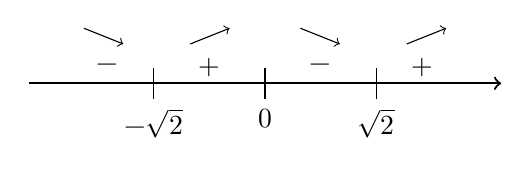
\begin{tikzpicture}
        % draw axis
        \draw [thick, ->] (-3, 0) -- (3, 0);

        % draw lines in x axis
        \draw (-1.41421356237, -0.2) -- (-1.41421356237, 0.2); % -sqrt(2)
        \draw (0,-0.2) -- (0,0.2); % zero
        \draw (1.41421356237, -0.2) -- (1.41421356237, 0.2); % sqrt(2)

        % write math symbols
        \node [below] at (-1.41421356237, -0.2) {$-\sqrt{2}$}; % -sqrt(2)
        \node [below] at (0,-0.2) {$0$};
        \node [below] at (1.41421356237, -0.2) {$\sqrt{2}$};

        % pluses-minuses
        \node at (-2, 0.2) {$-$};
        \node at (-0.70710678118, 0.2) {$+$};
        \node at (0.70710678118, 0.2) {$-$};
        \node at (2, 0.2) {$+$};

        % arrows
        \draw [->] (-2.3, 0.7) -- (-1.8, 0.5);
        \draw [->] (-0.95, 0.5) -- (-0.45, 0.7);
        \draw [->] (0.45, 0.7) -- (0.95, 0.5);
        \draw [->] (1.8, 0.5) -- (2.3, 0.7);
    \end{tikzpicture}
\end{figure}
\begin{gather*}
    f'(x)>0 \text{ при } x \in (-\sqrt{2};0); (\sqrt{2}; +\infty) \\
    f'(x)<0 \text{ при } x \in (-\infty; -\sqrt{2});(0;\sqrt{2})
\end{gather*}

3.
\begin{gather*}
    \begin{aligned}
        f(x) & =(x+2)^2 \sqrt{x} & \text{ОДЗ: }x & \geqslant 0 \\
    \end{aligned}\\
    f'(x)=2(x+2)\sqrt{x} + \frac{(x+2)^2}{2\sqrt{x}}=\frac{4x(x+2) + (x+2)^2}{2\sqrt{x}}=\frac{(x+2)(4x+x+2)}{2\sqrt{x}}\\
    \begin{aligned}
        x+2 & =0  & 5x+2 & =0             \\
        x   & =-2 & x    & = -\frac{2}{5} \\
    \end{aligned}
\end{gather*}
\begin{figure}[!h]
    \centering
    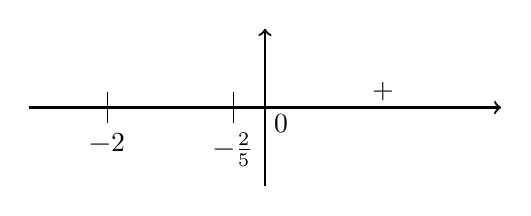
\begin{tikzpicture}
        % draw axis
        \draw [thick, ->] (-3, 0) -- (3, 0);
        \draw [thick, ->] (0, -1) -- (0,1);

        % draw lines in x axis
        \draw (-2, -0.2) -- (-2, 0.2); % -2
        \draw (-0.4, -0.2) -- (-0.4, 0.2); % -2/5
        \draw (0,-0.2) -- (0,0.2); % zero


        % write math symbols
        \node [below] at (-2, -0.2) {$-2$}; % -2
        \node [below] at (-0.4, -0.2) {$-\frac{2}{5}$}; %-2/5
        \node [right] at (0,-0.2) {$0$};

        % pluses-minuses
        \node at (1.5, 0.2) {$+$};
    \end{tikzpicture}
\end{figure}
\begin{gather*}
    x > 0\\
\end{gather*}
\subsection*{№826}
1.
\begin{gather*}
    f(x)=(5-3x)^4(3x-1)^3\\
    f'(x)=-12(5-3x)^3(3x-1)^3+9(3x-1)^2(5-3x)^4=0\\
    3(5-3x)^3 (3x-1)^2 (-4(3x-1)+3(5-3x))=0\\
    \begin{aligned}
        5-3x & =0            & 3x-1 & =0           & -12x+4+15-9x & =0             \\
        x    & =1\frac{2}{3} & x    & =\frac{1}{3} & x            & =\frac{19}{21} \\
    \end{aligned}
\end{gather*}
\begin{figure}[!h]
    \centering
    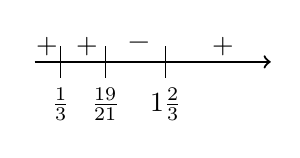
\begin{tikzpicture}
        % draw axis
        \draw [thick, ->] (0, 0) -- (3, 0);

        % draw lines in x axis
        \draw (1/3, -0.2) -- (1/3, 0.2);
        \draw (19/21, -0.2) -- (19/21, 0.2);
        \draw (5/3, -0.2) -- (5/3, 0.2);

        % write math symbols
        \node [below] at (1/3, -0.2) {$\frac{1}{3}$};
        \node [below] at (19/21, -0.2) {$\frac{19}{21}$};
        \node [below] at (5/3, -0.2) {$1\frac{2}{3}$};

        % pluses-minuses
        \node at (1/6, 0.2) {$+$};
        \node at (2/3, 0.2) {$+$};
        \node at (4/3, 0.2) {$-$};
        \node at (2.4, 0.2) {$+$};
    \end{tikzpicture}
\end{figure}
\begin{gather*}
    f'(x) <0 \\
    x \in (\frac{19}{21};1\frac{2}{3})
\end{gather*}

3.
\begin{gather*}
    \begin{aligned}
        f(x) & =\frac{3x^2 -1}{1-2x} & \text{ОДЗ: }1-2x & \neq 0           \\
             &                       & -2x              & \neq -1          \\
             &                       & x                & \neq \frac{1}{2}
    \end{aligned}\\
    f'(x)=\frac{6x(1-2x)-2(3x^2 -1)}{(1-2x)^2}\\
    6x-12x^2+-6x^2+2=0\\
    -6x+6x-2=0\\
    3x^2-3x+1=0\\
    D=9-4\cdot3\cdot1=-3\\
    f'(x)<0 {} x \in \mathbb{R} (x\neq \frac{1}{2})
\end{gather*}
\begin{gather*}
\end{gather*}
\end{document}